\section{SPIND Overview}\label{sec:spind}

We will now propose our algorithm \textit{SPIND}, which stands for \textbf{S}calable \textbf{P}artial \textbf{IN}clusion \textbf{D}ependency discovery. Further, the German word \textit{SPIND} is a special kind of closet, and often multiple "Spinds" are placed next to each other. This is a metaphor for the algorithm procedure. Every input relation will be transformed to a single "Spind" of sorted values with connected attributes, which are larger than a \textit{BINDER} bucket \cite{papenbrock2015divide}.  The total number of "Spinds", contrary to \textit{BINDER} buckets, will not grow exponentially with the candidate space but be constant over all nary layers. \textit{SPIND}'s operations on a relational level offer solutions to multiple problems that no other algorithm can solve. The architecture does not need to monitor main memory consumption or estimate the size of objects. \textit{BINDER} uses heuristics to estimate if the content of a file can be loaded without overflowing the available main memory. In some rare cases, this heuristic can fail, leading to an execution failure. Another issue is the creation of many files. For data sets with many (p)INDs, algorithms like \textit{BINDER} or \textit{SPIDER} will create at least one file per attribute regardless of the size of the data set \cite{papenbrock2015divide, bauckmann2006efficiently}. Especially in nary (p)IND discovery, these algorithms can create millions of files, which are all very small, creating massive I/O overhead. In addition to the problems that \textit{SPIND} solves, it also outperforms \textit{BINDER} and \textit{SPIDER} computationally by a factor of up to multiple magnitudes and enables the user more flexibility in deciding how \textit{NULL} entries and duplicates should be handled.

The following subsections will guide through \textit{SPINDs} execution cycle which is illustrated in Figure \ref{fig:spind}. Section \ref{subsec:chunking} will explain the procedure computed once at the start of the algorithm. We create horizontally spitted chunks for each relation to obtain parallelizable tasks with approximately equal complexity. The chunks are then sorted (Section \ref{subsec:spind_sort}), creating a set of inverted indices for each relation. All indices are than merged (Section \ref{subsec:spind_merge}) by performing a $k$-way merge. At the end of the main loop, we validate the pIND candidates, using our own parallel validation procedure (Section \ref{sec:spind_val}). The validated pINDs of the current layer are then used to generate the candidates for the next layer (Section \ref{sec:candidate_gen}). Section \ref{subsec:prob_filter} discusses how we build and query a probabilistic filter to reduce I/O operations by using knowledge of the value distribution in dependent attributes.

Our proposed methods are implemented such that they can be used for unary and nary discovery, which lowers complexity and potential points of failure. To understand how we enable the methods to support arbitrary pIND sizes, Section \ref{subsec:nary-strings} explains our serialization techniques.

\begin{figure}[t]
    \centering
    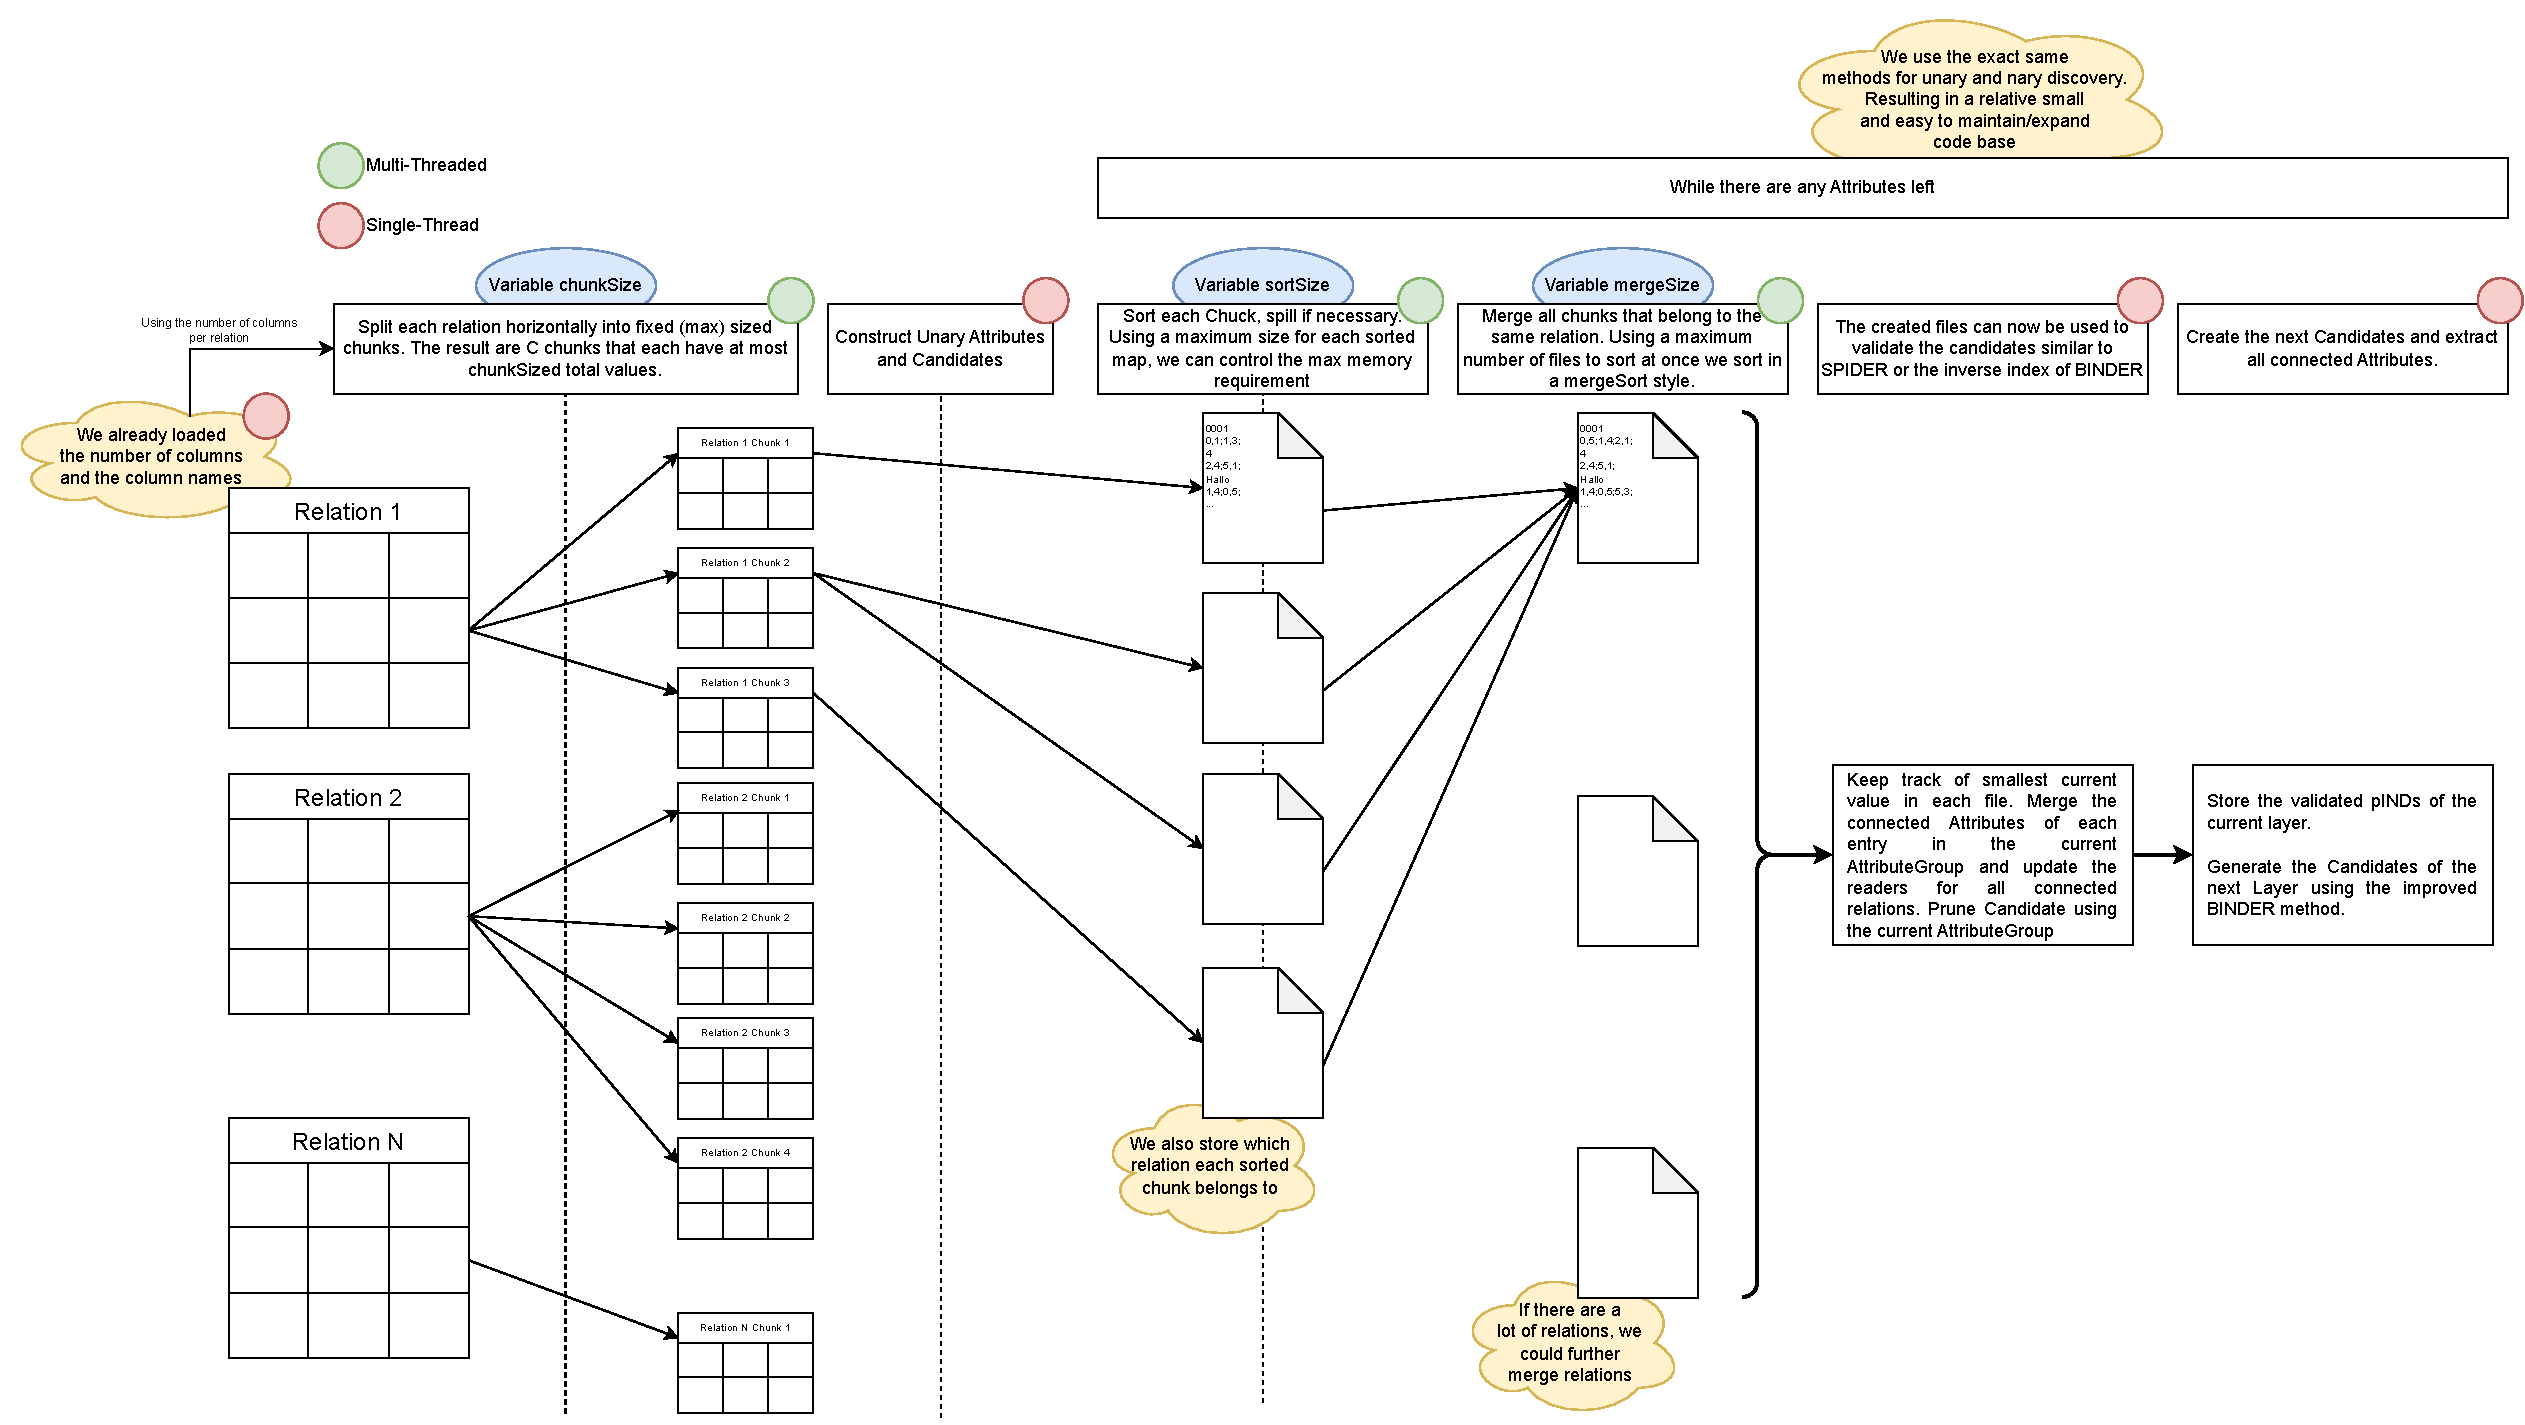
\includegraphics[width=0.4\textwidth]{figures/SPIND.pdf}
    \caption{Conceptual overview of \textit{SPIND}}
    \label{fig:spind}
\end{figure}

\subsection{Chunking the input relations}\label{subsec:chunking}
Modern CPUs feature multiple cores capable of performing tasks concurrently. Previous studies have largely overlooked the potential of parallelization \cite{smirnov2023fast, papenbrock2015divide, bauckmann2006efficiently, bell1995discovery}. In contrast, \textit{SPIND} will leverage parallelization extensively to maximize hardware utilization. Achieving this goal requires the identification of independent tasks that can be processed in parallel. \textit{SPINDs} execution starts by fetching some very basic information about the input relations. For each relational instance \textit{SPIND} will extract or generate the header column. Using a constant $CHUNK\_SIZE$ that is set by the user, we split each relation horizontally. Each chunk will consist of at most 
$$\#\textit{rows} = \left \lceil \frac{CHUNK\_SIZE}{\#\textit{columns}} \right \rceil$$
rows. The complexity of processing a relation directly correlates with the number of total values in that relation. While this may be an oversimplification since there are many more factors, like the distribution of duplicate values, the raw size is easy to modify and a heuristic that can be applied without any specific dataset knowledge. Each of the resulting chunks is associated with exactly one relation and carries a subset of rows. Chunking is performed once at the start of an execution and is not repeated for nary layers. We reuse the same chunks in every layer of the nary pIND discovery.

Since \textit{SPIND} almost always operates on the relation layer, a hash-based partitioning similar to \textit{BINDER} is not feasible. For the validation, we need to descend to the attribute layer and there we need to know which attributes share a given value. A partitioning would therefore be required to split the dataset into $n$ groups $G_1, \dots, G_n$ such that for every tuple of values $t_i$ generated by some row of a relation, it holds that if $t_i \in G_j$ then 
\begin{itemize}
    \item[1)] $\forall \: t_k \in G \setminus G_j : t_i \cap t_k = \emptyset$,
    \item[2)] $t_i \cap t_k \not = \emptyset \: \forall \: t_k \in G_j$.
\end{itemize}
To find such groups we would need knowledge of all values in a relation. Even if we expand the groups row by row and merge when necessary, solving this grouping problem would create a lot of new complexity. This leads to the decision to use a plain horizontal splitting approach.

After the chunking phase is complete, we obtain a collection of chunks for each relation. Larger relations are divided into more chunks, whereas smaller relations are likely to be contained within a single chunk, allowing for efficient parallel processing.

\subsection{Sorting Chunks} \label{subsec:spind_sort}
Our objective is to organize each chunk in ascending order, a necessary condition for the subsequent merging and validation processes. We build an inverted index which maps values to attributes they occur in additionally storing the values occurrence in that attribute. Each chunk is subjected to the same processing steps, executed in parallel.

We link a \textit{CSVReader}\footnote{Provided by the open source library "Opencsv" \url{https://opencsv.sourceforge.net/} (Last access: 05/06/2024)} to each chunk, specifying the relevant attributes. Each chunk is processed line by line, during which all related attributes are updated to their new values. The exact method for assigning values to nary attributes is detailed in Section \ref{subsec:nary-strings}. At this point, we will assume that there is an appropriate string representation available for both unary and nary tuples. We use a hash-based mapping structure to associate values with their corresponding attributes (attributes are referenced by an integer index) and track the frequency of occurrences, creating a nested map (in java style: Map<String, Map<Integer, Long>$\!\,$>). To avoid memory overflow, we limit the map's size using a constant called \textit{SORT\_SIZE}. When the map size hits the defined limit (which is divided by the number of threads) or when sorting is finished, the data within the map is serialized to disk.

First, we arrange the key set of the outer map in order. Next, we iterate through the sorted entries, writing two lines for each entry. The first line is the string representation of the value, which is the entry's key, followed by the attributes that constitute the value along with their frequencies. If there are $k$ attributes associated with a value, the attributes are serialized in the format $id_1,count_1;\dots;id_k,count_k$. For example, if the value "Marburg" appears twice in the attribute with id "1" and 40 times in the attribute with id "3", we would write "Marburg" on the first line and "1,2;3,40" on the second line. For each spilled file, we keep the path of the sorted inverted index and ultimately we return a list of these paths.

\subsection{Merging Inverted Indices}\label{subsec:spind_merge}
We currently have a set of individually sorted inverted indices, where each file from the same relation needs to be merged. This process is executed in parallel. To mitigate the issue of excessive file openings, the constant \textit{MERGE\_SIZE} is used to restrict the number of files being sorted at the same time. We attach a reader to each file and use a priority queue to perform a $k$-way merge \cite{taniar2008high}. At the end of the merge phase, we have constructed a single sorted file for each relation.

Modern SSDs, when used with buffered readers, can effectively eliminate I/O bottlenecks that previously constrained algorithm designs. Other researchers have also observed that SSDs, particularly when paired with parallel processing, can significantly enhance the performance of data processing algorithms \cite{meena2014performance}.

\subsection{Validation of Candidates}\label{sec:spind_val}
At this point of \textit{SPINDs} execution, we have constructed a single inverted index file for each relation. The validation procedure is similar to that of \textit{SPIDER}, but we implement it in parallel. With the sorted files, we identify attributes that have common values and incrementally advance the readers so that only those with the same smallest value are updated. \textit{SPIDER} uses a priority queue which stores the head value of each reader. Such a data structure enables us to calculate the smallest of the head values in $\log(|\mathcal{R}|)$ time for every insertion, $\mathcal{R}$ being the set of relational instances. Assume that the complexity of pruning candidates for some value is $\mathcal{O}(k)$. Computing the candidate pruning for all (distinct) values $N$ would cost $O(k \cdot N \cdot \log(|\mathcal{R}|))$. Pruning is a synchronous task, which means that active candidates need to be synchronized between every prune. We will therefore try to create the attribute groups in parallel and conduct pruning in the main thread.

\begin{figure}
    \centering
    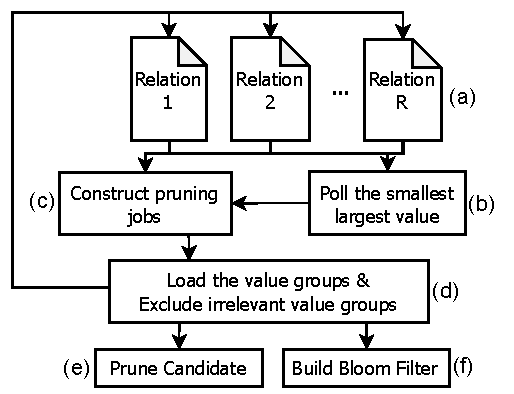
\includegraphics[width=.38\textwidth]{figures/multi_validation.pdf}
    \caption{Parallelized Validation on a relational level.}
    \label{fig:parallel_validation}
\end{figure}

We introduce the last variable \textit{VALIDATION\_SIZE}. It is a fixed value which states how many values are pre-loaded in total over all relation. In Figure \ref{fig:parallel_validation} we present our new parallelized approach to candidate pruning. Every pruning cycle starts by refilling the queue of every relation (Figure \ref{fig:parallel_validation}.a). The relation files are sorted and we read the ordered values until each queue reaches $$
\textit{queueSize} = \left \lfloor \frac{\textit{VALIDATION\_SIZE}}{|\mathcal{R}|} \right \rfloor. 
$$
The queues are filled in parallel. Once a reader reaches the end of its file and the queue has been completely emptied in the last cycle, we detach that reader. As a next step, we find the minimum over the last value in each queue (Figure \ref{fig:parallel_validation}.b). Using a queue with a first and last pointer, this can be calculated in $\mathcal{O}(|\mathcal{R}|)$ time. We store this smallest largest value. Using a hash-based map, with a capacity of \textit{VALIDATION\_SIZE} we will construct pruning jobs within the main thread (Figure \ref{fig:parallel_validation}.c). Knowing that the serialized attributes of different relations can not have overlapping ids, we simply append the serialized string representations that share the same value, creating a String-to-String map. Appending the serialized attributes is much faster than deserializing them and merging the HashMaps. Once all values of all queues, which are smaller than the smallest largest value, have been emptied into the map, we will start a parallel computation over the entry set of the map (Figure \ref{fig:parallel_validation}.d). For every entry of the map we first load the serialized attributes creating a \textit{valueGroup}, which maps attribute ids to occurrences and includes all attributes which share the given value. For each attribute we check, if the attribute is still a dependent part for any candidate ($\mathcal{O}(1)$) and if that is false we further check if the attribute acts as a referenced side for any attribute ($\mathcal{O}(1)$). Should both tests yield false, we remove the attribute from the \textit{valueGroup} since the given attribute has already been pruned from all candidates. Should no attribute of the group be part of a dependent side, we can skip pruning and will instead insert the given value into the probabilistic filter (Figure \ref{fig:parallel_validation}.f, see Section \ref{subsec:prob_filter}).
Deserialization is computed in parallel for all readers and we calculate the smallest largest value for each relation queue after they have been refilled. This largest smallest queue value is calculate at most $$\left \lceil\frac{N}{\textit{VALIDATION\_SIZE}}\right \rceil$$ times if all $N$ values distributed over the different relations where pairwise distinct. Each individual computation requires linear time with respect to the number of current relations ($\mathcal{O}(|\mathcal{R}|)$). The value groups are then also build in parallel using a stream architecture to efficiently include the synchronized pruning. The resulting complexity is  $$\mathcal{O} \left( k \cdot N + \left \lceil |\mathcal{R}| \cdot \frac{N}{\textit{VALIDATION\_SIZE}}\right \rceil \right ).$$ Should $|\mathcal{R}|$, the number of relations, be very large $\log(|\mathcal{R}|)$ would eventually yield a better theoretical complexity. But since $|\mathcal{R}|$ can be expected to be much smaller than the \textit{VALIDATION\_SIZE} and the proposed version operates mostly in parallel, we find that this concept of loading groups in parallel and already removing attributes which can not provide information decreases the compute time by a factor of up to five and especially helps when processing large datasets.

